%%% LaTeX Template: Two column article
%%%
%%% Source: http://www.howtotex.com/
%%% Feel free to distribute this template, but please keep to referal to http://www.howtotex.com/ here.
%%% Date: February 2011

%%% Preamble
\documentclass[	DIV=calc,%
							paper=a4,%
							fontsize=11pt,%
							twocolumn]{scrartcl}	 					% KOMA-article class

\usepackage{lipsum}													% Package to create dummy text

\usepackage[french]{babel}										% English language/hyphenation
\usepackage[protrusion=true,expansion=true]{microtype}				% Better typography
\usepackage{amsmath,amsfonts,amsthm}					% Math packages
\usepackage[pdftex]{graphicx}									% Enable pdflatex
\usepackage[svgnames]{xcolor}									% Enabling colors by their 'svgnames'
\usepackage[hang, small,labelfont=bf,up,textfont=it,up]{caption}	% Custom captions under/above floats
\usepackage{epstopdf}												% Converts .eps to .pdf
\usepackage{subfig}													% Subfigures
\usepackage{booktabs}												% Nicer tables
\usepackage{fix-cm}													% Custom fontsizes
\usepackage[utf8]{inputenc}
\usepackage[rightcaption]{sidecap} 
\usepackage{graphicx} %package to manage images
\usepackage{listings}
\usepackage{color}

\definecolor{mygreen}{rgb}{0,0.6,0}
\definecolor{mygray}{rgb}{0.5,0.5,0.5}
\definecolor{mymauve}{rgb}{0.58,0,0.82}

\lstdefinestyle{customc}{
  belowcaptionskip=1\baselineskip,
  breaklines=true,
  frame=L,
  xleftmargin=\parindent,
  language=C,
  showstringspaces=false,
  basicstyle=\footnotesize\ttfamily,
  keywordstyle=\bfseries\color{green!40!black},
  commentstyle=\itshape\color{purple!40!black},
  identifierstyle=\color{blue},
  stringstyle=\color{orange},
}

\lstdefinestyle{customasm}{
  belowcaptionskip=1\baselineskip,
  frame=L,
  xleftmargin=\parindent,
  language=[x86masm]Assembler,
  basicstyle=\footnotesize\ttfamily,
  commentstyle=\itshape\color{purple!40!black},
}

\lstset{escapechar=@,style=customc}

\lstset{ %
  language=C,
  backgroundcolor=\color{white},   % choose the background color; you must add \usepackage{color} or \usepackage{xcolor}
  basicstyle=\footnotesize,        % the size of the fonts that are used for the code
  breakatwhitespace=false,         % sets if automatic breaks should only happen at whitespace
  breaklines=true,                 % sets automatic line breaking
  captionpos=b,                    % sets the caption-position to bottom
  commentstyle=\color{mygreen},    % comment style
  deletekeywords={...},            % if you want to delete keywords from the given language
  escapeinside={\%*}{*)},          % if you want to add LaTeX within your code
  extendedchars=true,              % lets you use non-ASCII characters; for 8-bits encodings only, does not work with UTF-8
  frame=single,	                   % adds a frame around the code
  keepspaces=true,                 % keeps spaces in text, useful for keeping indentation of code (possibly needs columns=flexible)
  keywordstyle=\color{blue},       % keyword style
  language=Octave,                 % the language of the code
  otherkeywords={*,...},           % if you want to add more keywords to the set
  numbers=left,                    % where to put the line-numbers; possible values are (none, left, right)
  numbersep=5pt,                   % how far the line-numbers are from the code
  numberstyle=\tiny\color{mygray}, % the style that is used for the line-numbers
  rulecolor=\color{black},         % if not set, the frame-color may be changed on line-breaks within not-black text (e.g. comments (green here))
  showspaces=false,                % show spaces everywhere adding particular underscores; it overrides 'showstringspaces'
  showstringspaces=false,          % underline spaces within strings only
  showtabs=false,                  % show tabs within strings adding particular underscores
  stepnumber=2,                    % the step between two line-numbers. If it's 1, each line will be numbered
  stringstyle=\color{mymauve},     % string literal style
  tabsize=2,	                   % sets default tabsize to 2 spaces
  title=\lstname                   % show the filename of files included with \lstinputlisting; also try caption instead of title
}



%%% Custom sectioning (sectsty package)
\usepackage{sectsty}													% Custom sectioning (see below)
\allsectionsfont{%															% Change font of al section commands
	\usefont{OT1}{phv}{b}{n}%										% bch-b-n: CharterBT-Bold font
	}

\sectionfont{%																% Change font of \section command
	\usefont{OT1}{phv}{b}{n}%										% bch-b-n: CharterBT-Bold font
	}



%%% Headers and footers
\usepackage{fancyhdr}												% Needed to define custom headers/footers
	\pagestyle{fancy}														% Enabling the custom headers/footers
\usepackage{lastpage}	

% Header (empty)
\lhead{}
\chead{}
\rhead{}
% Footer (you may change this to your own needs)
\lfoot{\footnotesize \texttt{Thibaut EHLINGER, Benjamin HERB} \textbullet ~Systèmes distribués et grilles : TP1}
\cfoot{}
\rfoot{\footnotesize page \thepage\ of \pageref{LastPage}}	% "Page 1 of 2"
\renewcommand{\headrulewidth}{0.0pt}
\renewcommand{\footrulewidth}{0.4pt}



%%% Creating an initial of the very first character of the content
\usepackage{lettrine}
\newcommand{\initial}[1]{%
     \lettrine[lines=3,lhang=0.3,nindent=0em]{
     				\color{DarkGoldenrod}
     				{\textsf{#1}}}{}}



%%% Title, author and date metadata
\usepackage{titling}															% For custom titles

\newcommand{\HorRule}{\color{DarkGoldenrod}%			% Creating a horizontal rule
									  	\rule{\linewidth}{1pt}%
										}
										
										\renewcommand\thesubsubsection{}

\pretitle{\vspace{-15pt} \begin{flushleft} \HorRule 
				\fontsize{15}{15} \usefont{OT1}{phv}{b}{n} \color{DarkRed} \selectfont 
				}
\title{Systèmes distribués et grilles : TP1}					% Title of your article goes here
\posttitle{\par\end{flushleft}\vskip 0.1em}

\preauthor{\begin{flushleft}
					\large \lineskip 0.1em \usefont{OT1}{phv}{b}{sl} \color{DarkRed}}
\author{Thibaut EHLINGER, Benjamin HERB }											% Author name goes here
\postauthor{\footnotesize \usefont{OT1}{phv}{m}{sl} \color{Black} 
					Université de Strasbourg 								% Institution of author
					\par\end{flushleft}\HorRule}

\date{19 septembre 2016}																			



%%% Begin document
\begin{document}
\maketitle
\thispagestyle{fancy} 			% Enabling the custom headers/footers for the first page 
% The first character should be within \initial{}
\initial{L}\textbf{e} but de ce TP est de mettre en évidence l'impact de l'utilisation de \textit{clusters} de PC dans l'exécution d'un algorithme très gourmand en calcul, ici un produit de matrices. Dans un premier temps, nous présenterons rapidement notre résolution du problème pour le code manquant dans le projet. Puis nous présenterons les résultats des différents essais ; résultats que nous analyserons ensuite afin d'essayer de trouver quel est le choix le plus judicieux pour exécuter un produit de matrices de $ 4096 \times 4096 $ lignes.




\subsection*{Résultats}

\subsubsection*{Conditions d'expérimentation}
Les mesures de l'expérimentation n'ont été effectuées qu'une seule fois. Il est donc claire que ces résultats sont qualitatifs et non quantitatifs. Ce rapport sert surtout à mettre en avant un raisonnement. Les conclusions sont à prendre avec précautions et à revérifier expérimentalement sur plus d'essais. \newline
Nous nous sommes basés sur le temps d'exécution de la boucle pour les mesures de temps.

\subsubsection*{Kernel 1 contre kernel 0}
Bien que cela ne présente qu'un aspect mineur des performances de la machine que nous devions évaluer, il est tout de même intéressant de comparer les différences de performances entre les deux kernels. Cette différence est mise en exergue figure \ref{fig:diff_kern}, où l'on constate que le kernel 0 est bien plus lent que le kernel 1. Bien que l'échelle logarithmique estompe visuellement cette différence, elle permet de mettre en valeur la régularité de cette écart. Ainsi sur deux nœuds par exemple, on constate que le temps d'exécution sur le kernel 1 et 4 fois plus rapide environ que sur le kernel 0.  A noter que le kernel 0 met même plus de \textbf{deux minutes} avec un seul nœud à faire le calcul. 
\begin{figure}
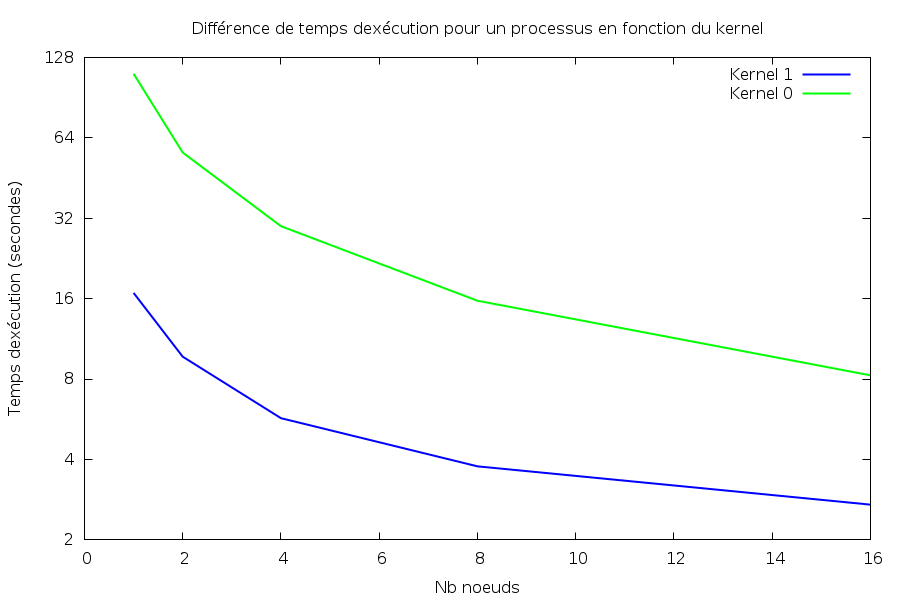
\includegraphics[keepaspectratio,width=8.5cm]{img/diff_kernels.png} 
\caption{Comparaison du temps d'exécution avec un seul processus entre les kernels 0 et 1.}
\label{fig:diff_kern}
\end{figure}

\subsubsection*{\textit{Round robin} contre une répartition voisine des tâches}
\begin{figure}
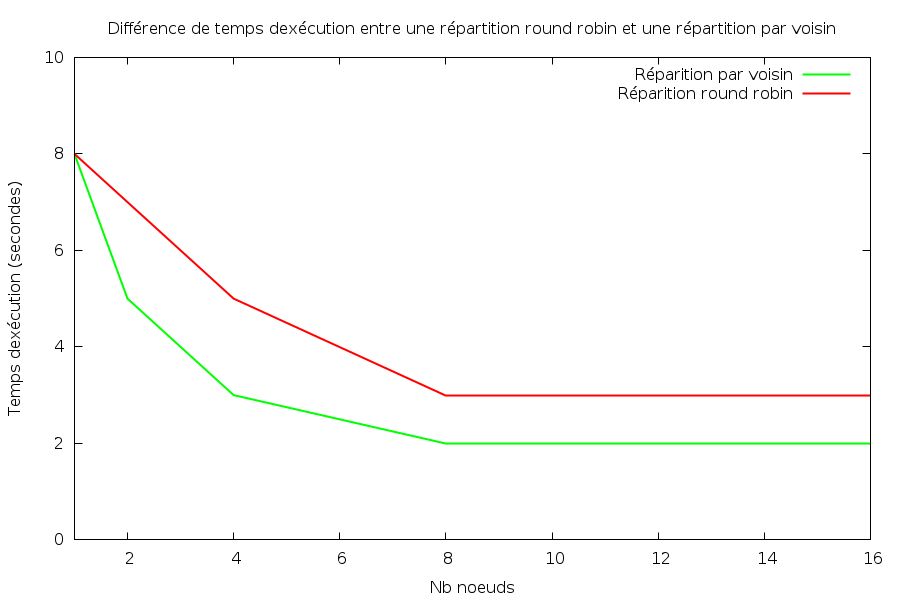
\includegraphics[keepaspectratio,width=8.5cm]{img/rr_v.png} 
\caption{Comparaison du temps d'exécution en round robin contre voisins pour 1 et 2 threads. Les performances sont \textit{évidemment} les mêmes pour un seul nœud.}
\label{fig:rr_v}
\end{figure}
Avec deux instance \textit{MPI} par nœud, il est très important de prêter attention à la répartition des instances MPI. En d'autres mots, on constate que la manière de répartir les instances sur les nœuds par paire influe grandement sur les résultats.\newline
Ici, nous avons choisi de nous intéresser à deux répartitions précises : \textit{round robin} contre une répartition de proche en proche, aussi appelée "\textit{par voisins}".\newline
En effet, dans l'algorithme, chaque instance MPI calcule une tranche de la matrice résultat à partir d'une tranche de la matrice $ \mathcal{A} $, puis il transfère cette tranche de $ \mathcal{A} $  à son voisin. C'est la localisation de ce voisin qui différencie les deux modes de répartition des instances MPI : en mode "\textit{par voisins}", on met les voisins sur un même nœud, tandis qu'en \textit{round robin}, on répartit les instances tour à tour sur les nœuds et c'est seulement après avoir attribué une instance par nœud qu'on recommence. Ainsi, ce sont à chaque fois des instances avec des identifiants très éloignées qui se retrouvent sur un  même nœud, ce qui fait que la circulation des tranches de $ \mathcal{A} $ nécessite bien plus de temps de communication.\newline
La figure \ref{fig:rr_v} met la différence de temps d'exécution en exergue. On constate que la répartition en \textit{round robin} est plus lente que la répartition en voisins quelque soit le nombre de noeuds, sauf évidemment pour \textbf{un noeud}, où le mode de répartition donne évidemment le même résultat.

\subsubsection*{Comparaison de l'efficacité en fonction des différents paramètres}
Pour cette problématique nous n'allons nous intéresser, pour les paires de processus par nœud, qu'au mode de répartition par voisins, celui-ci étant meilleur toutes choses égales par ailleurs au mode de répartition \textit{round-robin}. \newline
Est-il \textit{interéssant} d'utiliser deux threads par processus et deux processus par noeud au lieu de juste un thread par noeud et un noeud par processus?\newline
\textbf{De plus}, n'ayant effectué les mesures qu'une seule fois, il est claire que ces données ne peuvent en aucun cas être représentatives. Néanmoins la démarche employée serait la bonne pour un plus grand jeu de données.
\begin{figure}
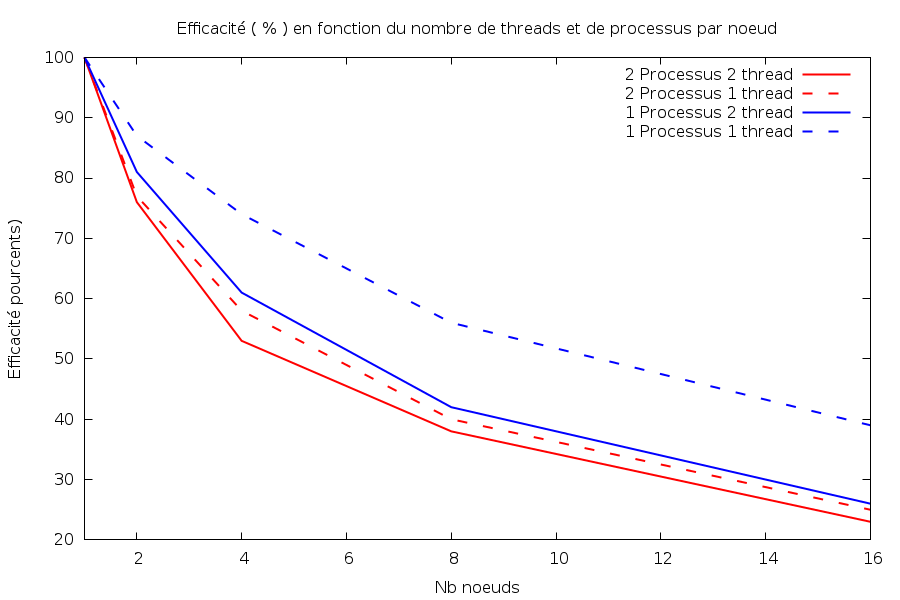
\includegraphics[keepaspectratio,width=8.5cm]{img/eff.png} 
\caption{Comparaison du temps de l'efficacité, en pourcents, en fonction du nombre de threads/processus par nœud. }
\label{fig:eff}
\end{figure}
Sur la figure \ref{fig:speed} on voit très clairement que le mode de calcul 1 processus/1 thread est beaucoup plus lent que les autres, en revanche départager les autres n'est pas évident car les courbes de la figure \ref{fig:eff} témoignent d'une efficacité très similaire en fonction du nombre de nœuds. Comme le temps de calcul ne  permet pas de repérer de très grande différence, nous nous baserons sur la puissance de calcul. La nature même de l'unité (le gigaflop) donne lieu à de plus grands écarts mis en évidence figure \ref{fig:power}. Sur celle-ci, on constate que la puissance est globalement similaire pour 1 processus/2 threads et 2 processus/2threads. En revanche il y a une grande "chute" de puissance chez 2 processus/1 thread  à 8 nœuds plus. Il faudrait reproduire plusieurs fois l'expérience pour savoir s'il s'agit d'une anomalie.
\begin{figure}
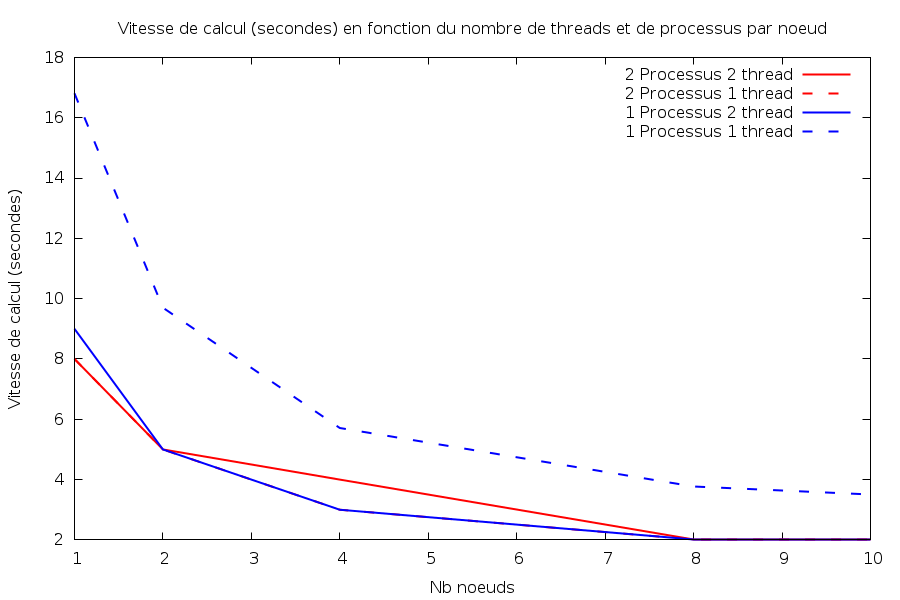
\includegraphics[keepaspectratio,width=8.5cm]{img/speed.png} 
\caption{Comparaison du temps de calcul en fonction du nombre de threads/processus par nœud.(On s'arrête à 8 nœuds car difficile de voir une différence au-delà)}
\label{fig:speed}
\end{figure}

\begin{figure}
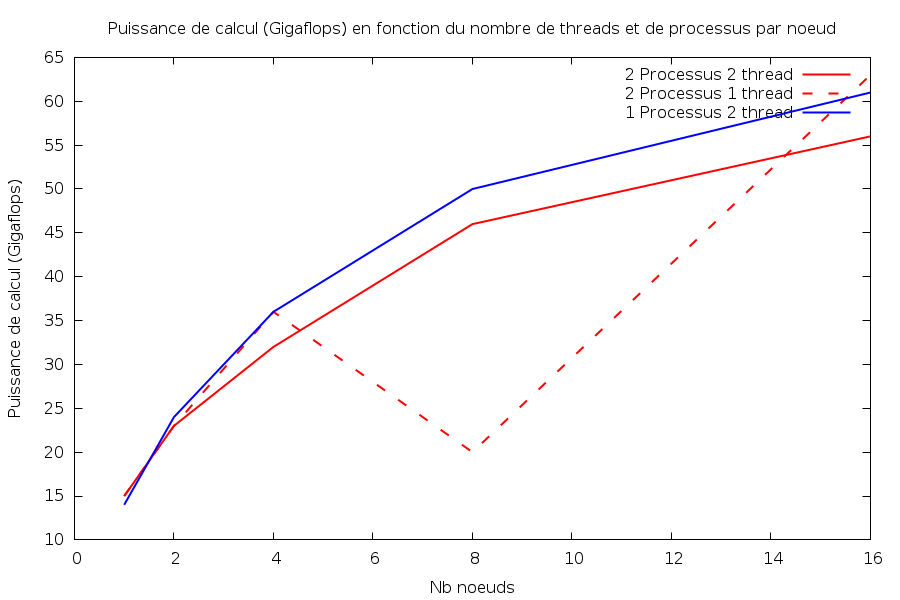
\includegraphics[keepaspectratio,width=8.5cm]{img/power.png} 
\caption{Comparaison de la puissance (gigaflops) en fonction du nombre de threads/processus par nœud.}
\label{fig:power}
\end{figure}

\subsubsection*{Tendances déduites des résultats}
Pour résumer, on peut conclure qu'il assez certain : 
\begin{itemize}
\item que le kernel 0 est bien moins efficace que le kernel 1 ;
\item que la répartition en round robin est bien moins efficace que la répartitions par voisins.
\end{itemize}
Les premiers résultats, qu'il faudrait compléter avec plus de données, laissent à penser, que : 
\begin{itemize}
\item le mode 1 thread/1 processus est clairement moins bon que les autres. ;
\item il est presque toujours rentable d'utiliser 2 threads au lieu de 1 thread;
\item il difficile de trouver le meilleur compromis entre 2 threads/2 processus, 2 threads/ 1 processus et 2 processus / 1 thread. Dans ce contexte, j'aurai tendance à prendre le mode de calcul le \textbf{moins gourmand}, ou en tout cas à éliminer le plus gourmand, c'est à dire 2 threads 2 processus.
\end{itemize}

\section*{Résolution du problème}
Dans un premier temps, nous devions compléter trois parties spécifiques du code, qui concernaient l'initialisation MPI, le calcul de l'\textit{offset} de départ dans la matrice pour chacun de processus en fonction de leur identifiant MPI, et enfin les différentes étapes de la boucle principale, c'est à dire l'échange des données et le calcul des sous-parties de la matrice résultat par chaque processus. Cette partie se décompose en deux sous-fonctions : \texttt{ComputationAndCirculation} et \texttt{OneStepCirculation}.

\subsection*{Initialisation MPI}
\begin{lstlisting}
#include <stdio.h>
#define N 10

/* Initialisation of processor coordinates */

void ProcessorInit(void){
	MPI_Comm_size(MPI_COMM_WORLD,&NbPE);
  	MPI_Comm_rank(MPI_COMM_WORLD,&Me);
}
\end{lstlisting}

\newpage

\subsection*{Calcul de l'offset pour un processus {\texttt{Me} donné}}
\begin{lstlisting}
/* Compute the current step offset, in the MPI program, to access right C lines */ OffsetStepLigC = ((Me + step) * LOCAL_SIZE) % SIZE; 
\end{lstlisting}

\subsection*{Boucle principale}
\begin{lstlisting}
void ComputationAndCirculation()
{
 unsigned long step;
 
 for(step=0;step<NbPE;step++) { 
  OneLocalProduct(step);
  OneStepCirculation(step);
 }
}
/* Elementary circulation of A and B.                                            */
void OneStepCirculation(unsigned long step)
{
 MPI_Status   status;

 MPI_Sendrecv_replace(A_Slice, SIZE*LOCAL_SIZE, MPI_DOUBLE, (Me-1+NbPE)%NbPE, 0, (Me+1)%NbPE, 0, MPI_COMM_WORLD, &status);
}


\end{lstlisting} 
\end{document}